% Paper 1 — Radio Science (AGU) manuscript draft
% Compile from this directory: pdflatex paper1_radioscience.tex (twice)
\documentclass[draft]{agujournal2025}

\begin{document}

\journalname{Radio Science}

\title{Series Sheath Capacitance of a Plasma-Immersed Dipole in Three-Dimensional Fluid FDTD: Volumetric Jacket Versus Analytic Coaxial Loading}

\authors{%
S.~Neshragh\affil{1}%
% Add coauthors as needed, e.g.: , A.~Coauthor\affil{1,2}
}

\affiliation{1}{Department / Institution (update before submission)}

\authoraddr{%
S.~Neshragh, corresponding author address and email (update before submission)
}

\authorrunninghead{Ignored.}
\titlerunninghead{Ignored.}

\keypoints%
{A prescribed vacuum jacket around a dipole in 3D fluid FDTD acts as series sheath capacitance, not a shunt feed capacitor.}%
{Low-frequency CW shows Im\{Z\} zero-crossings falling with sheath width, opposite to a dielectric-unloading upward-shift scoreboard.}%
{Band-averaged C\_eff(Sd) tracks coaxial analytic C\_sh(Sd) in trend with a nearly constant scale factor near 0.3 for Sd = 2 and 10.}

\maketitle

\begin{abstract}
We quantify how a prescribed volumetric vacuum sheath of width \(S_d\) cells loads the feed impedance of a thin-wire dipole in a three-dimensional plasma-fluid finite-difference time-domain (PF-FDTD) solver. After attaching the sheath to the conductor (PEC-seeded density depletion), continuous-wave (CW) phasor measurements at plasma frequency \(f_p=2\,\mathrm{MHz}\) show strong \(S_d\) dependence of \(Z(f)\). Using the first \(\mathrm{Im}\{Z\}\) positive-to-negative crossing as a series-resonance marker yields \(f_\mathrm{res}(0)\approx 1.85\,\mathrm{MHz}\), \(f_\mathrm{res}(2)\approx 0.66\,\mathrm{MHz}\), and \(f_\mathrm{res}(10)\le 0.50\,\mathrm{MHz}\): the crossing moves downward with sheath thickness. We interpret this as series sheath capacitance \(1/(j\omega C_\mathrm{sh})\) dominating dielectric unloading. Defining an effective capacitance \(C_\mathrm{eff}=-1/(\omega\,\mathrm{Im}\{Z\})\) on capacitive branches and averaging over \(0.8\)--\(1.2\,\mathrm{MHz}\) gives \(C_\mathrm{eff}(2)\approx 7.4\,\mathrm{pF}\) and \(C_\mathrm{eff}(10)\approx 4.3\,\mathrm{pF}\). These values decrease with \(S_d\) in the same sense as a coaxial analytic sheath \(C_\mathrm{sh}=2\pi\varepsilon_0 L/\ln(1+S_d\Delta x/r_\mathrm{eff})\) with Holland-like \(r_\mathrm{eff}=0.23\Delta x\), with \(C_\mathrm{eff}/C_\mathrm{sh}\approx 0.30\) at both thicknesses. The work provides a quantitative bridge between volumetric FDTD sheaths and Balmain/Liu-type series gap models used for plasma impedance probes, and clarifies why an upward \(f_\mathrm{res}(S_d)\) target inspired by transmitting-antenna sheath literature is the wrong scoreboard for a static prescribed jacket.
\begin{plainlanguagesummary}
Radio antennas in space plasmas sit inside a thin empty ``sheath'' next to the metal. We simulated that empty layer as a jacket of controlled thickness around a dipole in a 3-D plasma wave code. Making the jacket thicker made the antenna look more capacitive and moved its resonance to lower frequency, which matches treating the jacket as a series capacitor. The effective capacitance we extracted from the simulations decreases with jacket thickness in the same way as a simple coaxial capacitor formula, up to a nearly constant scale factor. This helps connect detailed wave simulations to the circuit models used to interpret plasma impedance probes.
\end{plainlanguagesummary}
\end{abstract}

\section{Introduction}

A conducting antenna immersed in plasma is surrounded by a depleted sheath that can dominate low-frequency impedance. Classical short-dipole theory in a cold magnetoplasma \cite{balmain1964,balmain1969} provides the homogeneous-medium baseline; later Balmain-era and contemporary treatments add ion sheaths, insulating jackets, and sheath-wave physics as series gap loading between metal and exterior plasma. Modern plasma impedance probe (PIP) retrievals often write an explicit coaxial sheath capacitor in series with a Balmain-like plasma term \cite{liu_pip}, so that the phase-zero frequency lies below bulk plasma features.

High-voltage transmitting antennas raise a related but distinct problem: Song and coworkers modeled an oscillating ion-sheath radius about a bare dipole \cite{song2007}, and Tu et al.\ used one-dimensional particle-in-cell (PIC) simulations to refine sheath structure and reactance \cite{tu2008}. Those studies motivate the statement that ``sheath changes antenna impedance,'' but they do not prescribe a fixed vacuum jacket in three-dimensional fluid FDTD, nor do they require that an \(\mathrm{Im}\{Z\}=0\) marker climb with sheath thickness.

This paper addresses a narrower, quantitative question suited to the PF-FDTD solver used here: does a \emph{prescribed} volumetric vacuum jacket of width \(S_d\Delta x\) behave as a \emph{series} sheath capacitor whose effective \(C_\mathrm{eff}(S_d)\) tracks coaxial analytic expectations? Campaign diagnostics that established conductor-attached sheath coupling and the downward \(f_\mathrm{res}(S_d)\) trend are summarized only as needed; the methodological path (including a pre-fix seeding bug) is documented elsewhere \cite{paper0}. Success is defined by \(C_\mathrm{eff}\) versus coax and multi-marker reporting of \(Z(f)\), not by an upward Im-zero shift with \(S_d\).

\section{Methods}

\subsection{PF-FDTD solver and antenna geometry}

PF-FDTD advances Maxwell's equations on a staggered Yee grid coupled to multi-species fluid continuity and momentum equations. Plasma current enters Ampere's law; feed observables are voltage \(V(t)\) and current \(I(t)\) at a hard \(E_z\) source, with
\begin{equation}
Z(f)=\frac{V(f)}{I(f)}
\end{equation}
from steady-state CW phasors on the last 50\% of each \texttt{.vc} record.

All runs use a \(70\times 70\times 65\) grid with \(\Delta x=0.04\,\mathrm{m}\) and a \(z\)-directed thin-wire dipole from grid indices \((35,35,20)\) to \((35,35,45)\) (length \(L=1.00\,\mathrm{m}\)) with the feed at \((35,35,33)\). Unless noted, \(f_p=2\,\mathrm{MHz}\), collisions are weak, and the background magnetic field is zero.

\subsection{Prescribed volumetric sheath}

Ambient density is initialized uniformly, then depleted in a shell of width \(S_d\) cells about PEC cells (\(\mathrm{ER}_x\mathrm{ER}_y\mathrm{ER}_z=0\)):
\begin{equation}
0 < d \le S_d
\quad\Rightarrow\quad
N_0 \rightarrow N_0\cdot 10^{-6},
\end{equation}
so plasma current is negligible and the jacket behaves as vacuum. Sheath seeding from the plasma-on mask (rather than PEC) previously placed depletion at the domain boundary and made \(Z\) independent of \(S_d\); all results here use the PEC-seeded implementation \cite{paper0}.

\subsection{CW campaigns}

Two CW grids share the same geometry and \(f_p\):
\begin{description}
\item[Dense band] \(S_d\in\{0,2,4,6,8,10\}\), \(f=1.50\)--\(2.30\,\mathrm{MHz}\) (100~kHz and selected half steps; 66 cases).
\item[Low-frequency extension] \(S_d\in\{0,2,10\}\), \(f=0.50\)--\(1.50\,\mathrm{MHz}\) (100~kHz steps), to locate crossings for \(S_d\ge 2\).
\end{description}
Series resonance \(f_\mathrm{res}\) is the first \(\mathrm{Im}\{Z\}\) positive-to-negative zero crossing by linear interpolation. We also retain $|Z|$ structure as a second marker and do not equate phase-zero with magnitude extrema.

\subsection{Effective capacitance and coaxial reference}

Where \(\mathrm{Im}\{Z\}<0\), define
\begin{equation}
C_\mathrm{eff}(f)=-\frac{1}{\omega\,\mathrm{Im}\{Z(f)\}},
\qquad \omega=2\pi f.
\label{eq:ceff}
\end{equation}
This \(C_\mathrm{eff}\) is an \emph{effective} feed capacitance of the full antenna--sheath--plasma system, not a pure vacuum gap to an ideal plasma electrode. Band averages use \(0.8\)--\(1.2\,\mathrm{MHz}\) (capacitive points only), away from the narrow inductive island of \(S_d=2\) near \(0.60\,\mathrm{MHz}\).

The coaxial analytic sheath for a cylinder of length \(L\) and effective radius \(r_\mathrm{eff}\) is
\begin{equation}
C_\mathrm{sh}^\mathrm{(coax)}=\frac{2\pi\varepsilon_0 L}{\ln\!\bigl(1+S_d\Delta x/r_\mathrm{eff}\bigr)}.
\label{eq:coax}
\end{equation}
We take \(r_\mathrm{eff}=0.23\Delta x\) as a Holland-type thin-wire estimate on the Yee lattice \cite{holland1981}; sensitivity to \(r_\mathrm{eff}\) is discussed in Section~\ref{sec:disc}.

\section{Results}

\subsection{Impedance spectra and sheath coupling}

Figure~\ref{fig:zlow} shows low-frequency \(\Re\{Z\}\) and \(\mathrm{Im}\{Z\}\) for \(S_d=0,2,10\). Curves remain strongly separated ($|\Delta Z|/|Z_0|$ typically 80--350\%), confirming that the volumetric jacket enters the feed. \(S_d=0\) stays inductive through \(0.50\)--\(1.50\,\mathrm{MHz}\); \(S_d=10\) is capacitive at every low-frequency point; \(S_d=2\) is capacitive except for a brief inductive island at \(0.60\,\mathrm{MHz}\).

\begin{figure}
\noindent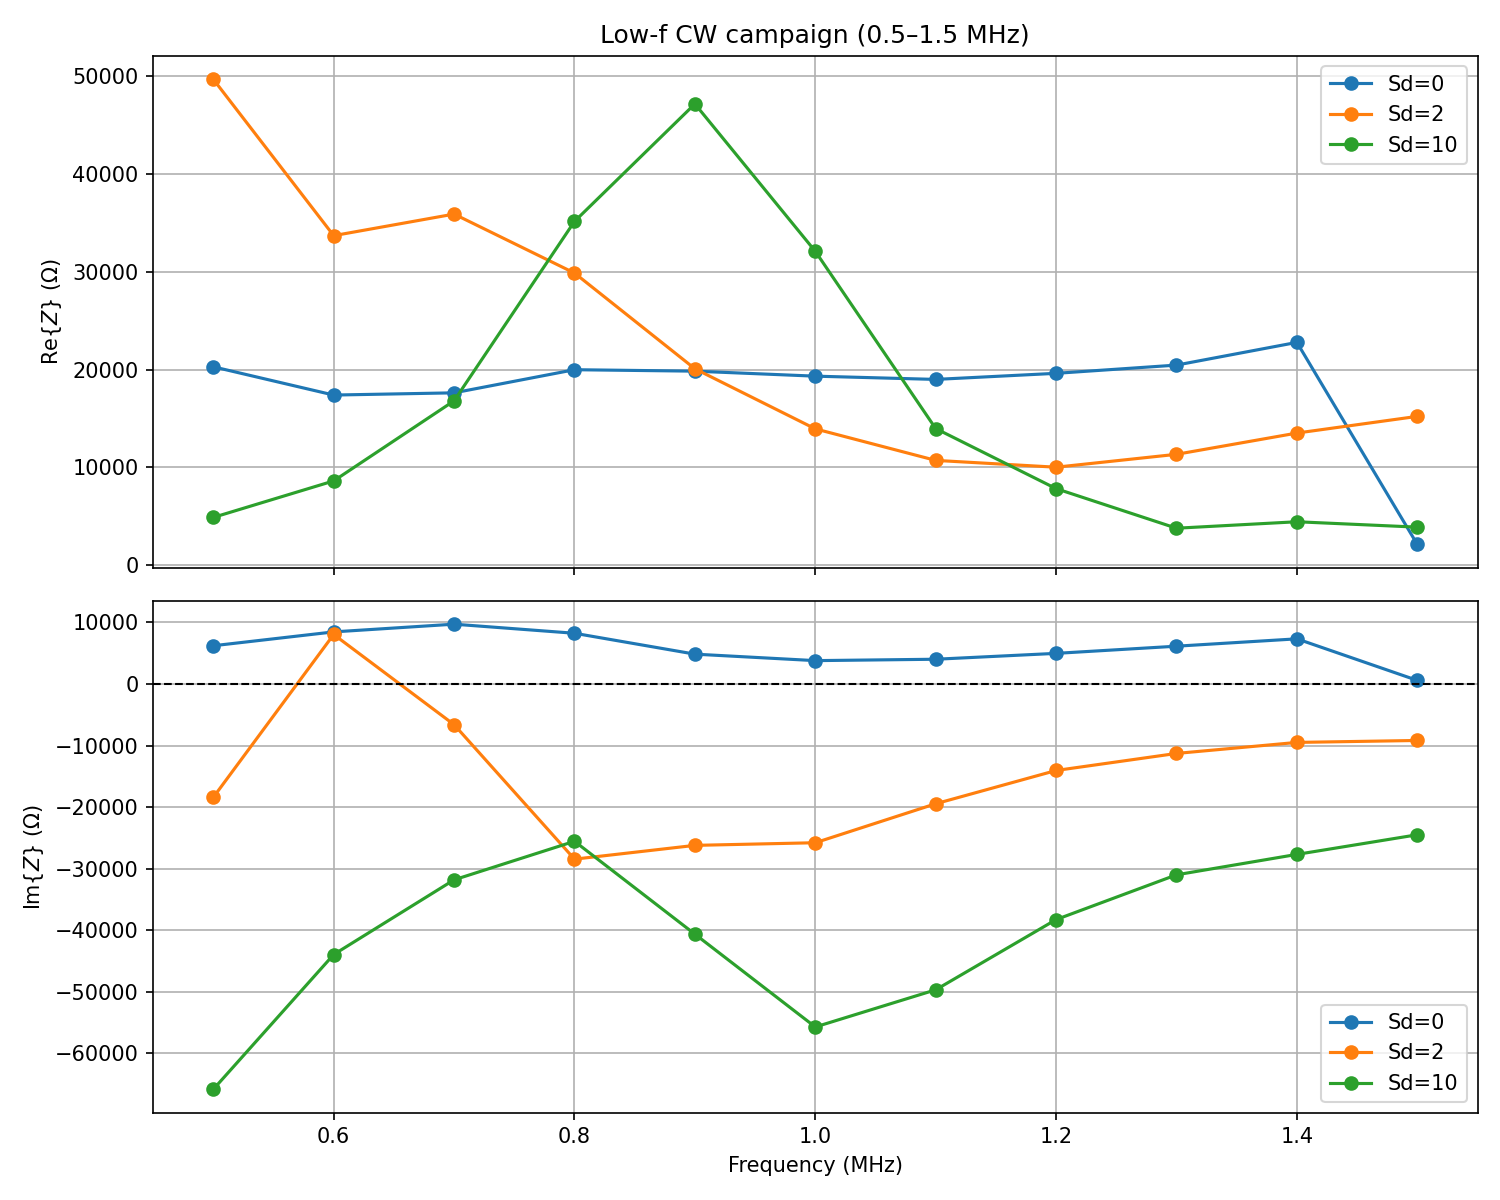
\includegraphics[width=\textwidth]{figures/cw_lowf_impedance_zoom.png}
\caption{Low-frequency CW phasor impedance for \(S_d=0,2,10\) (\(f_p=2\,\mathrm{MHz}\)). Top: \(\Re\{Z\}\); bottom: \(\mathrm{Im}\{Z\}\). The outlier at \(S_d=0\), \(1.50\,\mathrm{MHz}\) is an incomplete restart file and is discarded for physics.}
\label{fig:zlow}
\end{figure}

Figure~\ref{fig:zfull} combines the low-frequency extension with the dense high band. For \(S_d\ge 2\), \(\mathrm{Im}\{Z\}\) remains negative through \(1.50\)--\(2.30\,\mathrm{MHz}\); only \(S_d=0\) shows a high-band inductive-to-capacitive transition near \(1.85\,\mathrm{MHz}\).

\begin{figure}
\noindent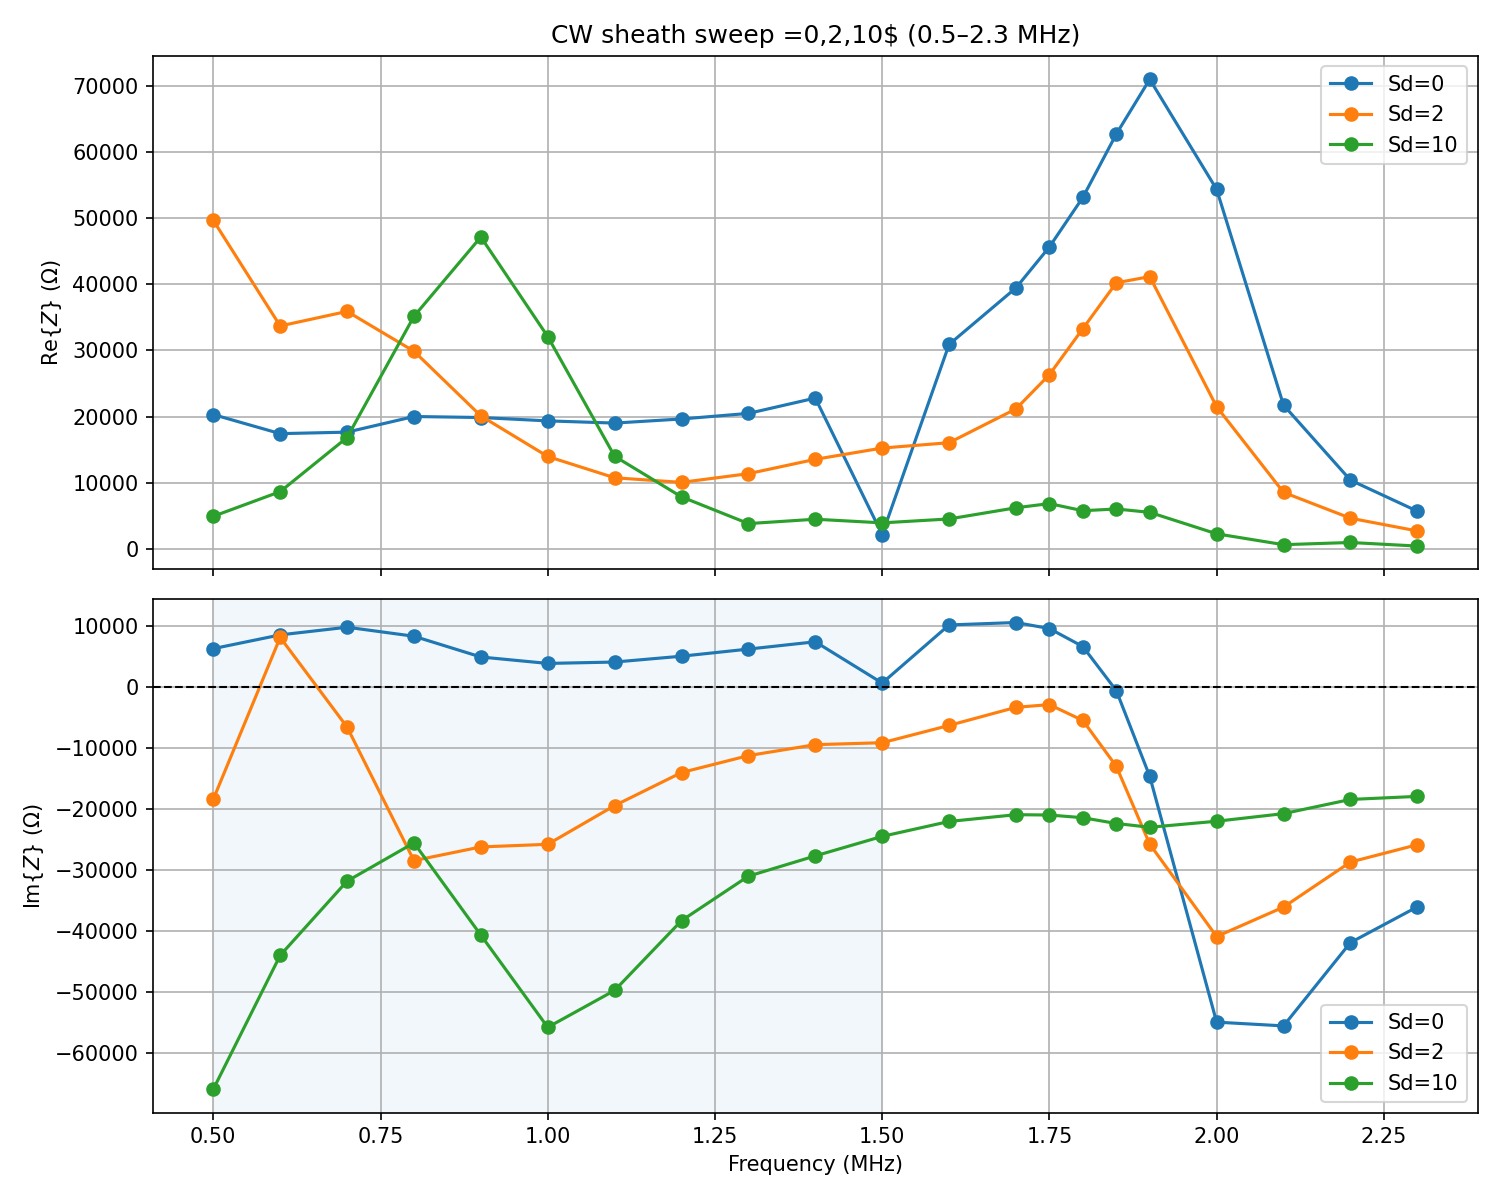
\includegraphics[width=\textwidth]{figures/cw_lowf_impedance.png}
\caption{Combined CW impedance for \(S_d=0,2,10\) over \(0.50\)--\(2.30\,\mathrm{MHz}\). The shaded region marks the low-frequency extension.}
\label{fig:zfull}
\end{figure}

\subsection{Resonance markers versus sheath width}

Table~\ref{tab:fres} and Figure~\ref{fig:fres} summarize \(\mathrm{Im}\{Z\}\) positive-to-negative crossings. Widening the jacket moves \(f_\mathrm{res}\) \emph{downward}, opposite to a dielectric-unloading upward-shift expectation for static \(S_d\).

\begin{table}
\caption{Series resonance from \(\mathrm{Im}\{Z\}\) \(+\) to \(-\) crossings}
\centering
\begin{tabular}{cll}
\hline
\(S_d\) & \(f_\mathrm{res}\) & Note \\
\hline
0 & \(1.846\,\mathrm{MHz}\) & August high band; low-frequency band all inductive \\
2 & \(0.655\,\mathrm{MHz}\) & Also \(-\) to \(+\) at \(0.570\,\mathrm{MHz}\) (inductive island) \\
10 & \(\le 0.50\,\mathrm{MHz}\) & All \(\mathrm{Im}\{Z\}<0\) in \(0.50\)--\(1.50\,\mathrm{MHz}\) \\
\hline
\end{tabular}
\label{tab:fres}
\end{table}

\begin{figure}
\noindent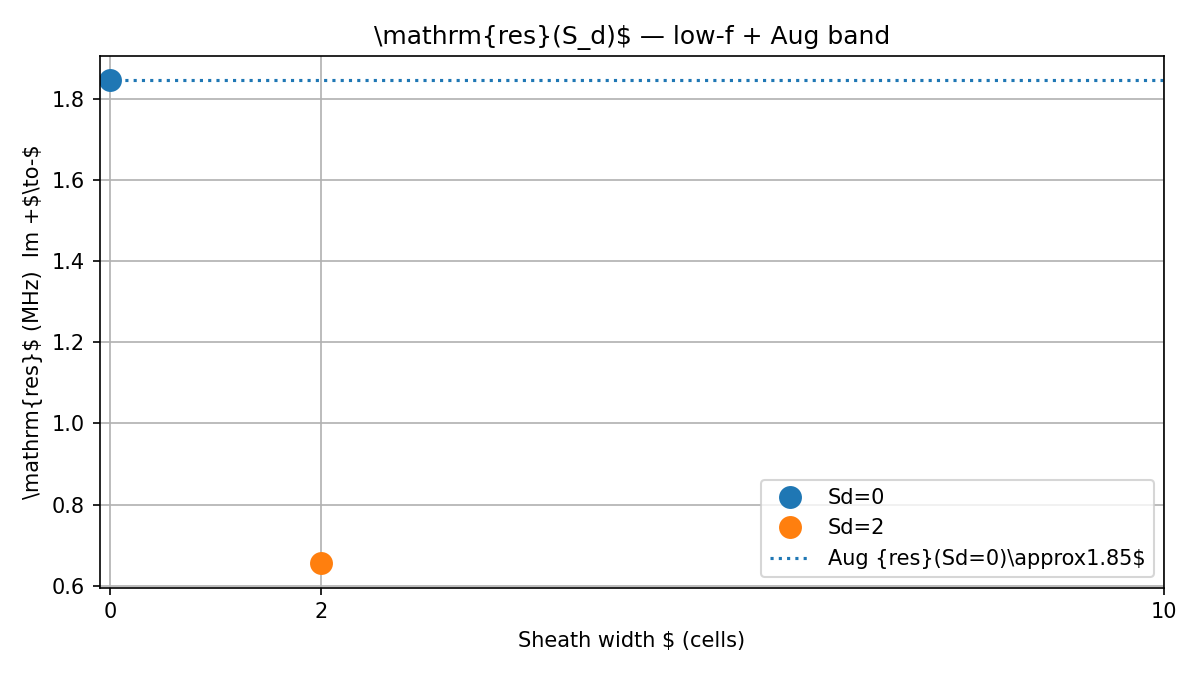
\includegraphics[width=0.85\textwidth]{figures/cw_lowf_resonance.png}
\caption{Resonance frequency \(f_\mathrm{res}(S_d)\) from \(\mathrm{Im}\{Z\}\) positive-to-negative crossings. \(S_d=10\) lies at or below the lower band edge.}
\label{fig:fres}
\end{figure}

\subsection{Effective capacitance versus coaxial sheath}

Figure~\ref{fig:cefff} shows \(C_\mathrm{eff}(f)\) from equation~(\ref{eq:ceff}) on capacitive branches. Band means over \(0.8\)--\(1.2\,\mathrm{MHz}\) are listed in Table~\ref{tab:ceff} and compared with equation~(\ref{eq:coax}) in Figure~\ref{fig:ceffsd}.

\begin{table}
\caption{Band-averaged \(C_\mathrm{eff}\) (\(0.8\)--\(1.2\,\mathrm{MHz}\)) versus coaxial \(C_\mathrm{sh}\)}
\centering
\begin{tabular}{ccccc}
\hline
\(S_d\) & \(t_\mathrm{sh}\) (m) & \(C_\mathrm{eff}\) (pF) & \(C_\mathrm{sh}^\mathrm{(coax)}\) (pF) & Ratio \\
\hline
2 & 0.08 & \(7.35\pm 1.12\) & 24.49 & 0.30 \\
10 & 0.40 & \(4.27\pm 1.83\) & 14.66 & 0.29 \\
\hline
\end{tabular}
\label{tab:ceff}
\end{table}

\begin{figure}
\noindent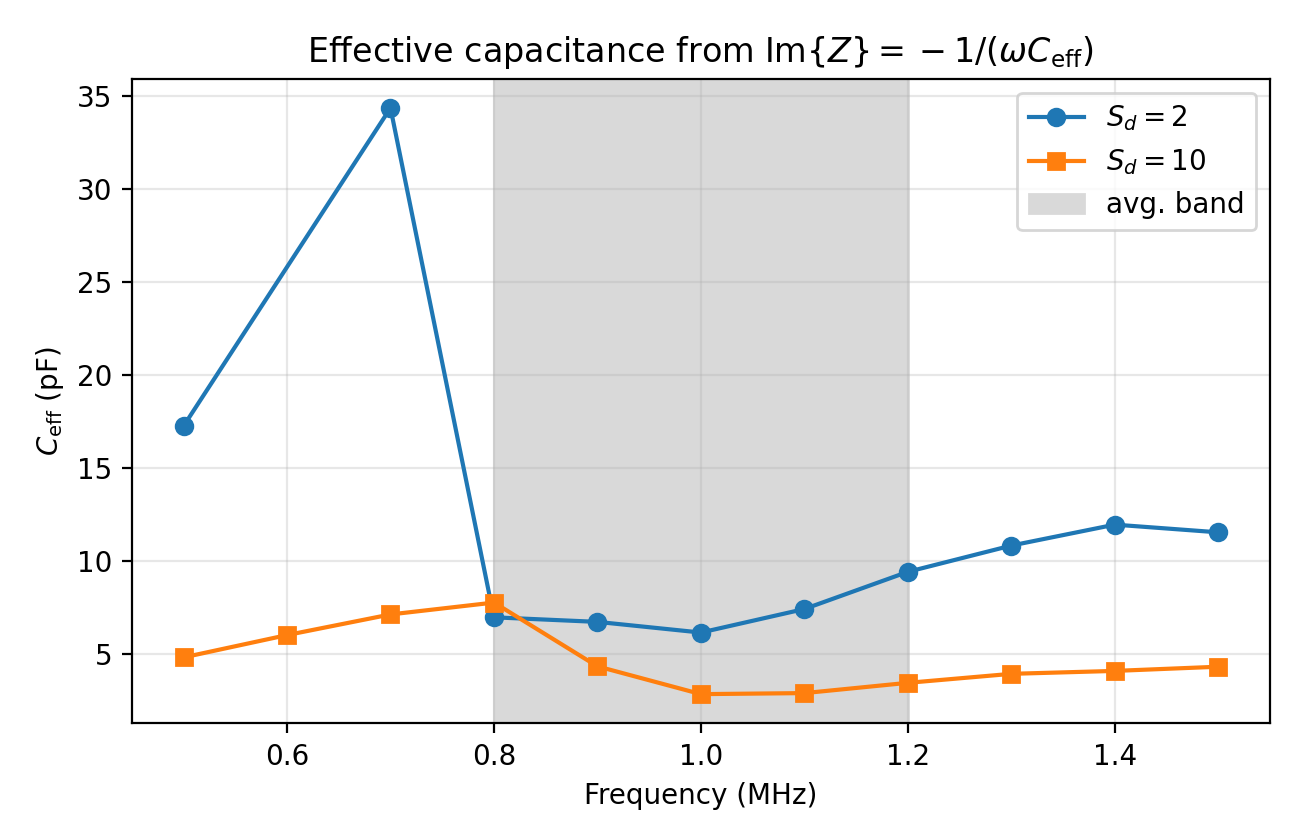
\includegraphics[width=0.85\textwidth]{figures/ceff_vs_frequency.png}
\caption{Effective capacitance \(C_\mathrm{eff}(f)\) for \(S_d=2\) and \(10\). Shaded band marks the averaging window used in Table~\ref{tab:ceff}.}
\label{fig:cefff}
\end{figure}

\begin{figure}
\noindent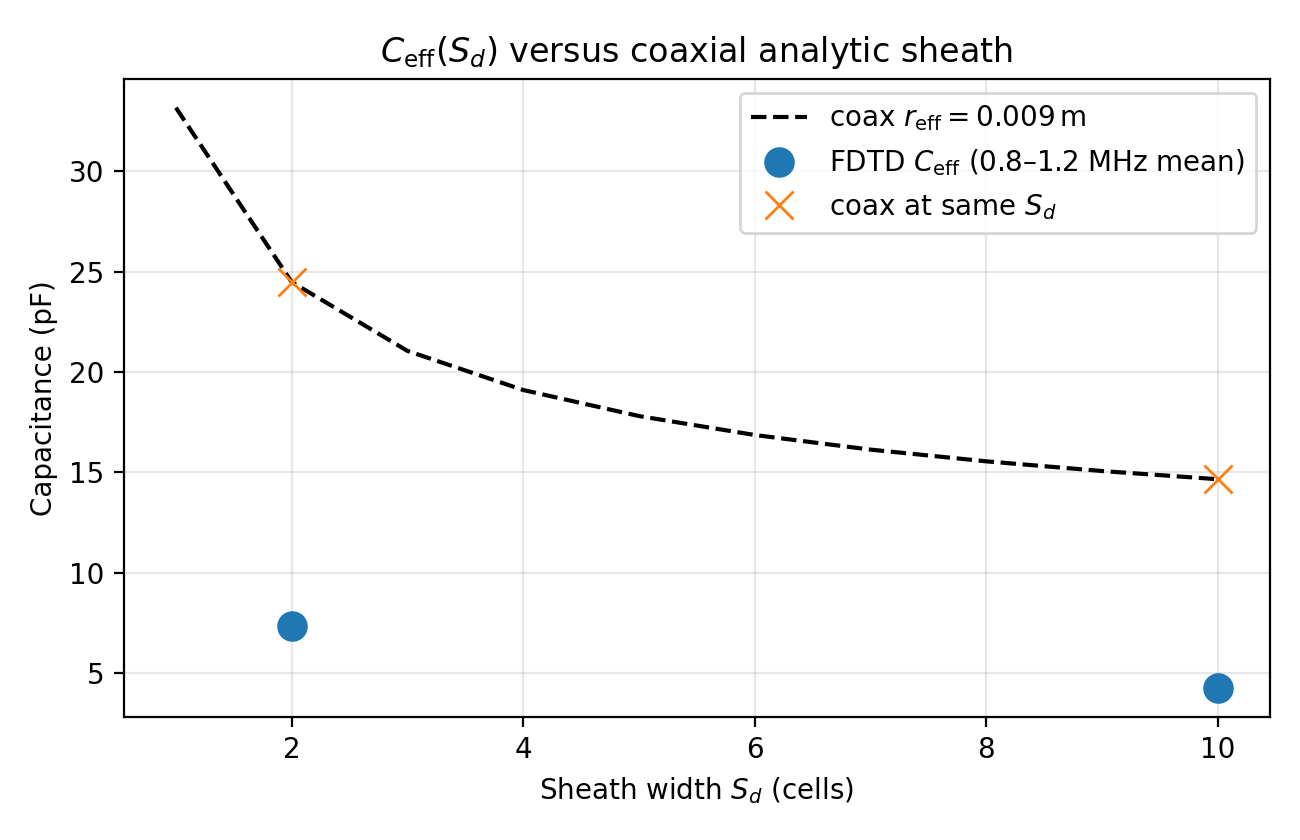
\includegraphics[width=0.85\textwidth]{figures/ceff_vs_coax.png}
\caption{\(C_\mathrm{eff}(S_d)\) (symbols) compared with coaxial analytic \(C_\mathrm{sh}(S_d)\) for \(r_\mathrm{eff}=0.23\Delta x\) (dashed). Crosses mark coax evaluated at the simulated \(S_d\).}
\label{fig:ceffsd}
\end{figure}

Both thicknesses show \(C_\mathrm{eff}<C_\mathrm{sh}^\mathrm{(coax)}\) by a nearly common factor \(\approx 0.30\). Absolute scale therefore depends on \(r_\mathrm{eff}\), staircasing, and residual plasma reactance inside \(C_\mathrm{eff}\), but the \emph{trend} with \(S_d\) matches series coaxial loading: thicker jackets reduce capacitance and strengthen capacitive reactance at fixed frequency.

\section{Discussion}
\label{sec:disc}

\subsection{Series versus parallel topology}

The depleted shell sits between the conductor and bulk plasma. Feed current must cross the gap by displacement current, so sheath loading appears in series with the plasma-loaded antenna impedance,
\begin{equation}
Z_\mathrm{in}(f)\approx Z_\mathrm{pl}(f)+\frac{1}{j\omega C_\mathrm{sh}(S_d)},
\end{equation}
not as a shunt capacitor across the terminals. Parallel-plate estimates \(C\sim\varepsilon_0 A/(S_d\Delta x)\) are pedagogical magnitude guides for that \emph{series} gap; they do not imply parallel circuit topology. Thin-wire geometry favors the logarithmic coax form (equation~(\ref{eq:coax})).

\subsection{Why \(f_\mathrm{res}\) falls with \(S_d\)}

Thickening the jacket simultaneously (i) removes plasma dielectric near the wire (favoring an upward shift toward free space) and (ii) inserts series \(C_\mathrm{sh}\) (favoring a downward phase-zero shift, as in PIP \(f_{\phi0}\) arguments). Under the \(\mathrm{Im}\{Z\}\) crossing metric on this grid, series capacitance wins. On \(\Delta x=0.04\,\mathrm{m}\), \(S_d=2\) is already an \(8\,\mathrm{cm}\) vacuum jacket---a strong capacitive load relative to a physical Debye sheath---which amplifies series-\(C\) domination.

\subsection{Relation to Tu et al.\ and Song et al.}

Tu \cite{tu2008} and Song \cite{song2007} address high-voltage transmitting dipoles with self-consistent, time-varying sheaths. The present runs prescribe a static step jacket in fluid FDTD. We therefore do not claim Tu dynamic fidelity. The appropriate static bridge is \(C_\mathrm{sh}(r_s)\) (and later, in follow-on work, prescribed \(\dot{r}_s\)), not an upward Im-zero scoreboard.

\subsection{Limitations}

\begin{enumerate}
\item Free-space \(f_\mathrm{res}\) on the same dipole remains an open upper anchor for the unloading narrative.
\item \(C_\mathrm{eff}\) mixes sheath and plasma reactance; a pure gap extraction would require additional modeling (e.g., vacuum reference or circuit de-embedding).
\item Absolute coax comparison depends on \(r_\mathrm{eff}\); the reported ratio \(\approx 0.3\) is for \(r_\mathrm{eff}=0.23\Delta x\). Larger \(r_\mathrm{eff}\) raises \(C_\mathrm{sh}\) further; smaller \(r_\mathrm{eff}\) improves absolute agreement but does not change the shared \(S_d\) trend.
\item Campaigns here are effectively unmagnetized; PIP upper-hybrid markers require \(B\neq 0\).
\item Only \(S_d=2\) and \(10\) enter the low-frequency \(C_\mathrm{eff}\) table; intermediate widths were capacitive in the dense band but were not re-run below \(1.5\,\mathrm{MHz}\).
\end{enumerate}

\section{Conclusions}

A prescribed volumetric vacuum sheath in PF-FDTD loads a plasma-immersed dipole as a \textbf{series} capacitor. CW measurements show \(\mathrm{Im}\{Z\}\) zero-crossings decreasing with \(S_d\), and band-averaged \(C_\mathrm{eff}(S_d)\) decreasing in parallel with coaxial analytic \(C_\mathrm{sh}(S_d)\) at nearly constant scale factor \(\approx 0.3\) for \(S_d=2\) and \(10\). These results validate series-gap loading as the correct FDTD interpretation of a static jacket and provide the quantitative baseline needed before prescribing time-varying sheath boundaries or self-consistent charging.

%%
%% Acknowledgments / Open Research (AGU required sections)
%%
\section*{Acknowledgments}
% Funding and thanks (update before submission).
The authors thank collaborators on the PF-FDTD sheath campaign for discussions of coupling diagnostics and impedance markers.

\section*{Open Research}
Simulation outputs supporting the figures are archived under the campaign results tree (\texttt{results/sheath\_cw\_tu/}) and derived tables in \texttt{paper1\_static\_sheath\_capacitance/analysis/data/}. Analysis scripts include \texttt{make\_ceff\_products.py}. Solver source is available in the collab PF-FDTD repository (branch with PEC-seeded \texttt{ApplySheath}). Update this section with a persistent DOI/repository link before submission.

\begin{thebibliography}{99}

\bibitem[Balmain(1964)]{balmain1964}
Balmain, K.~G. (1964), The impedance of a short dipole antenna in a magnetoplasma,
\textit{IEEE Trans. Antennas Propag.}, \textit{12}(5), 605--617,
doi:10.1109/TAP.1964.1138278.

\bibitem[Balmain(1969)]{balmain1969}
Balmain, K.~G. (1969), Dipole admittance for magnetoplasma diagnostics,
\textit{IEEE Trans. Antennas Propag.}, \textit{17}(3), 389--392,
doi:10.1109/TAP.1969.1139426.

\bibitem[Holland and Simpson(1981)]{holland1981}
Holland, R., and L.~Simpson (1981), Finite-difference analysis of EMP coupling to thin struts and wires,
\textit{IEEE Trans. Electromagn. Compat.}, \textit{EMC-23}(2), 88--97.

\bibitem[Liu et al.() ]{liu_pip}
Liu, et~al., Sheath-aware measurement uncertainty for plasma impedance probes,
manuscript under review. % Update citation upon publication.

\bibitem[Song et al.(2007)]{song2007}
Song, P., B.~W.~Reinisch, and et~al. (2007), High-voltage antenna--plasma interaction in whistler wave transmission: Plasma sheath effects,
\textit{J. Geophys. Res.}, \textit{112}, A06225,
doi:10.1029/2006JA011683.

\bibitem[Tu et al.(2008)]{tu2008}
Tu, W., P.~Song, and B.~W.~Reinisch (2008), Plasma sheath structures around a radio frequency antenna,
\textit{J. Geophys. Res.}, \textit{113}, A07223,
doi:10.1029/2008JA013097.

\bibitem[Ward(2006)]{ward2006}
Ward, J.~D. (2006), Plasma frequency probe design and implementation,
Master's thesis, Utah State University, Logan, Utah.

\bibitem[Paper0 campaign()]{paper0}
Neshragh, S., et~al., PF-FDTD sheath campaign chronicle and coupling diagnostics (2026),
internal report: \texttt{projects/tu2008-sheath/paper0\_sheath\_campaign/} and
\texttt{validation/phase\_7\_documentation/main.pdf}. % Replace with DOI when archived.

\end{thebibliography}

\end{document}
